\documentclass[technical_document.tex]{subfiles}
\begin{document}
Eva\textquotesingle s aesthetic design is based on the final concept drawing that was made. See figure \ref{fig:final_design}  The model was split into two parts of different complexity: the head part and the body part. Both parts were redesigned and converted to a 3-dimensional model. The redesigning was necessary to account for placement of internal parts, producability and the functioning of Eva. It was also thought that due to the rather sluggish  appearance of the final concept drawing the product character would not be familial - the desired product character. This is why the general design has been slimmed down. Firstly, the head was redesigned, for it has a considerable role in the manner of interaction of Eva. Secondly the body was redesigned; figure \ref{Eva} shows a render and a picture of the complete design of Eva.

\begin{figure}[h]
	\centering
	\mbox{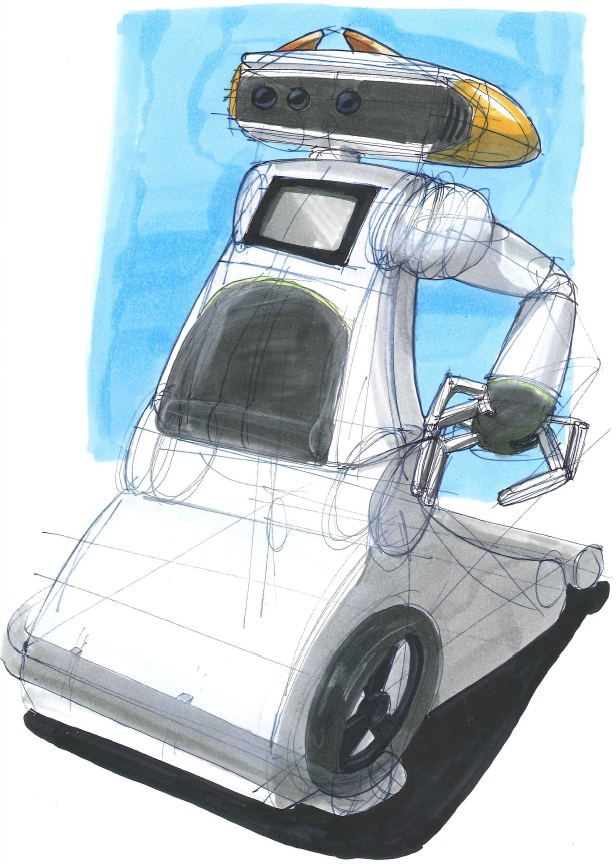
\includegraphics[width=0.5\textwidth]{Images/Final_Design.png}}
	\caption{Final aesthetic design of Eva}
	\label{fig:final_design}
\end{figure}

 \begin{figure}[h!]
  \centering
  \subfloat[Rendering of Eva.]
  {\label{fig:render_eva}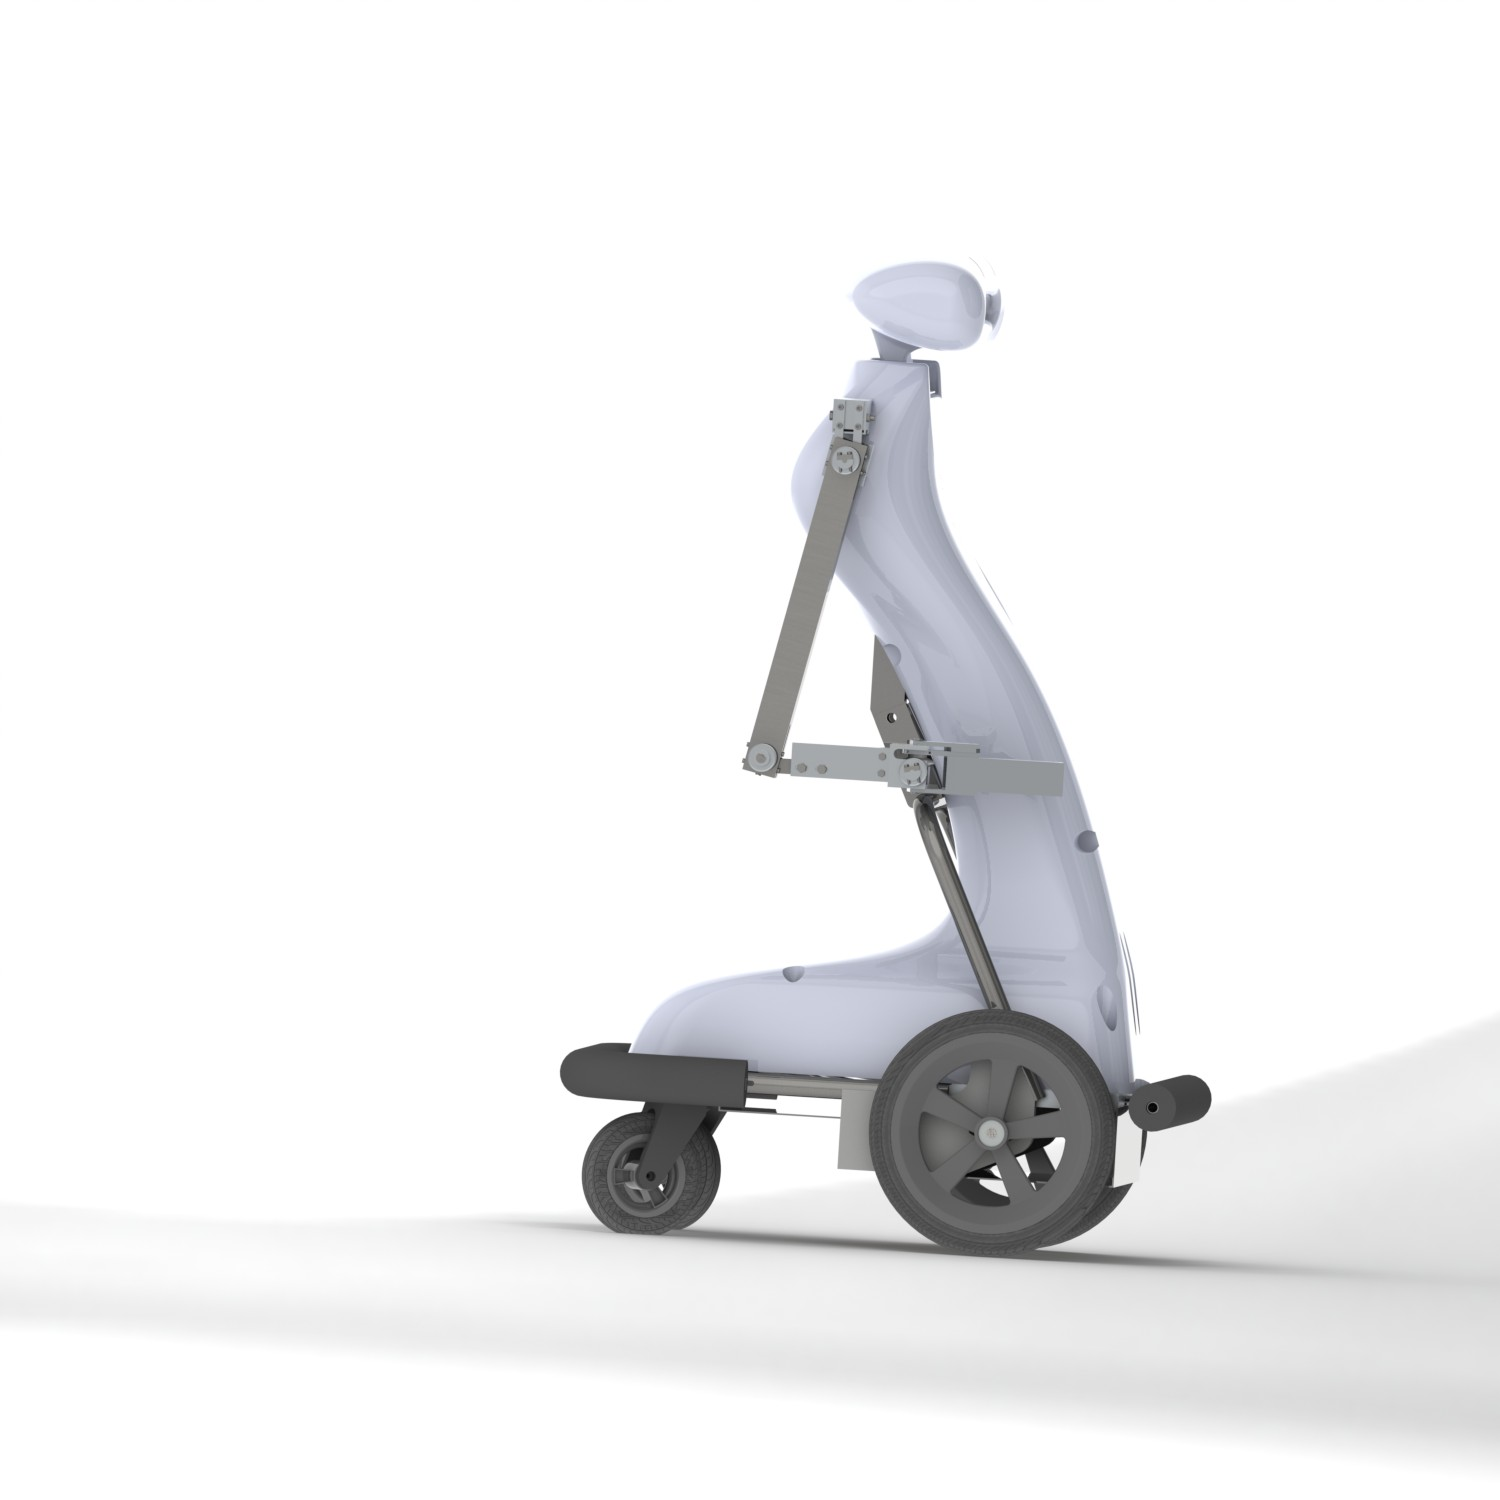
\includegraphics[width=0.45\textwidth]{Images/SW_almostfullrender.png}}    
  \hspace{2mm}            
  \subfloat[Photo of Eva]{\label{fig:photo_eva}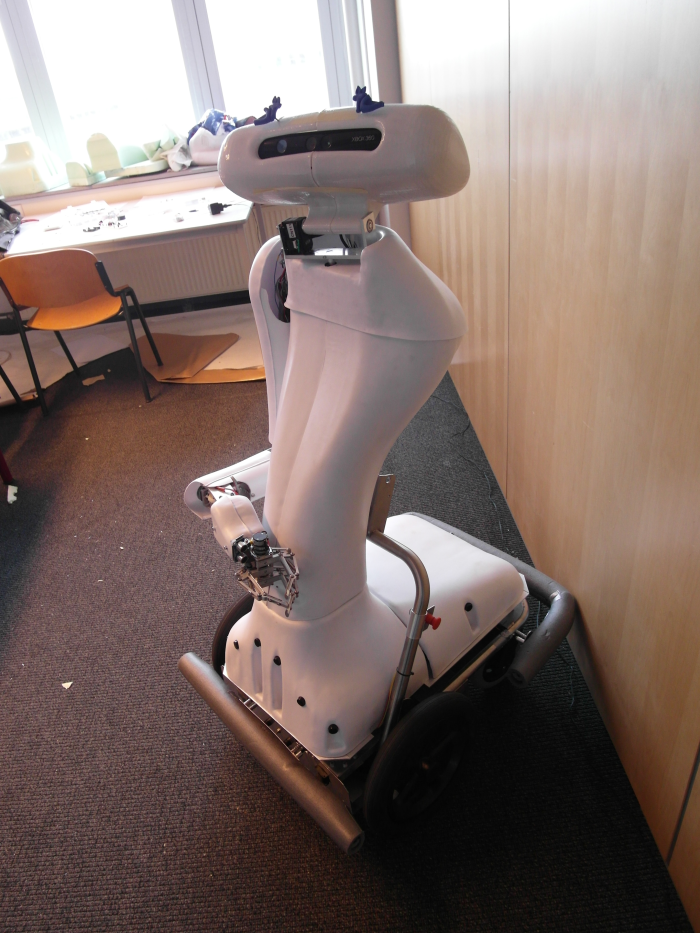
\includegraphics[width=0.3\textwidth]{Images/Evacomplete.png}}
  \caption{Images of Eva.}
  \label{Eva}
\end{figure}

\section{Head design}
\subsection*{Design considerations}
The head was redesigned foremost based on the demands of emotion display. This means that the design had to be thin enough 
to allow the RGB LEDs to shine through and allow placement of eyebrows that could move vertically and rotational. The 
design was also largely influenced by the demand that the kinect had to be returned intact at the end of the project. The 
other redesign demands were that all the parts had to be housed in the head, that the parts could be connected to the body 
by cables and that the head could be tilted by a motor later on. If possible we wanted  to place the speakers in the head, 
but that idea was rejected for it would change the size of the design too much. Due to a lack of testing material it could only be assumed that the light would shine through based on images on the web (see figure \ref{fig:finger} ) and a message 
from an employee of the production company Shapeways. This employee reported that with a $1 mm$ thickness the material would 
be translucent enough for LEDs to shine through.

\begin{figure}[h]
	\centering
	\mbox{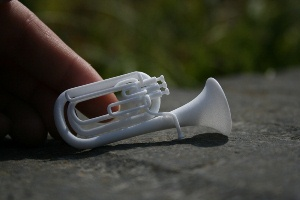
\includegraphics[width=0.5\textwidth]{Images/polish_horn_finger_thumb.png}}
	\caption{The light shines through the material}
	\label{fig:finger}
\end{figure}

\subsection{Production}
A 3D CAD model was made with a $0.8 mm$ wall-thickness. This thickness was chosen because it lays beneath the transluscent threshold of $1 mm$ and it allowed for a considerable decrease in price when compared with the original $1 mm$ design. It was known that this thickness would have a considerable influence on the strength of our design, but it was assumed that it could be strengthened after delivery by other materials. An actual simulation of forces exerted on the design could not be made since our simulation software Solidworks could not handle the complex curvatures in the design. Figure \ref{fig:head} shows the design of the head. Since the part was small and quite complex it was dicussed with an experts of the course Advanced Prototyping which manner of production would fit the design best. Ir. E.L. Doubrovski advised for the use of the 3-dimensional printing technique based on the size, complexity of the product and the speed of production. After redesigning the part based on his advice (splitting the model into two parts to allow part placement), the model was sent to Shapeways to print. The two parts are shown in figure \ref{fig:parts} .

\begin{figure}[h]
	\centering
	\mbox{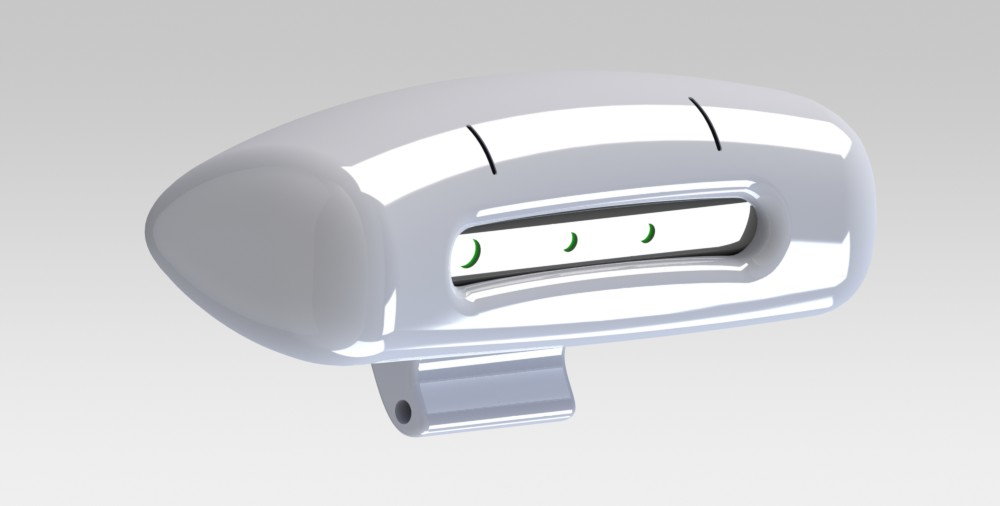
\includegraphics[width=0.5\textwidth]{Images/SW_fullheadmodel.png}}
	\caption{The design of the head part.}
	\label{fig:head}
\end{figure}

 \begin{figure}[h!]
  \centering
  \subfloat[One part of the head.]
  {\label{fig:render_head}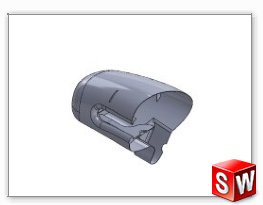
\includegraphics[width=0.46\textwidth]{Images/SW_halfmodel1.PNG}}    
  \hspace{2mm}            
  \subfloat[The other part of the head.]{\label{fig:photo_head}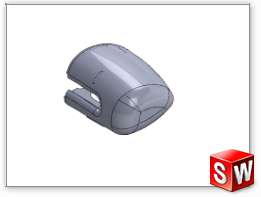
\includegraphics[width=0.45\textwidth]{Images/SW_halfmodel2.PNG}}
  \caption{Pictures of the head, split in two parts.}
  \label{fig:parts}
\end{figure}

\subsection{Design evaluation}
The design of the head made it difficult to assemble the head. The main reason was the very thin material needed to allow the light emitted from the RGB LEDs to shine through. This thinness made the head to deform easily and this made it difficult to fasten the head. This was solved by applying an epoxy-resin to stiffen the model and by placing supports from other materials in the model. An improvement would be to redesign the head to include non-permanent fasteners such as small bolts, which can be attached and detached easily. In the current design there is a lack of those non-permanent fasteners which means that we had to rely on tape to fasten the model. The vertically splitted face should also be changed to a horizontally splitted face. This would result in less difficulty when assembling. These changes would allow faster and easier access to the contents of the head. This does mean that a new method of fixing the Microsoft Kinect is needed. The current design allows the Kinect to be placed and fixed between the two sections; a horizontal split would remove this possibility. The wall thickness should also be made variable: thin on the sides to make the material translucent for the LEDs, but thicker in the middle to make the structure more rigid. A complete redesign of the inside of the model is also needed to ensure no additional material is needed for the placement of the Kinect and other parts. With the internal redesign some calculations should be made to know what kind of motor is needed for the tilting. When redesigning one can then ensure that the motor can fit inside the head. The currently used Dynamixel motor is too large and has to be placed outside the head.

\section{Main body design}
\subsection{Design considerations}
The main design consideration for the main body was the usage of the mobile base that was delivered by the minor organisation. The body also had to house the internal arm mechanism. A size estimate of these parts was made at the start of the design process. The arm covers were designed at a latter stage to accomodate the final design of the arm.

\subsection{Production} 
The covers were made using a thermoforming technique because of the low costs and the availability of the technique in the machine hall in the faculty of Industrial Design. Furthermore the covers could be divided in drafted parts without too much difficulty. Drafted parts are necessary for thermoforming.

A 3d CAD model of the mold was made based on the final drawing. This CAD model was then machined in the machine hall. This model then served as the positive mold for the thermoforming process. The mold was treated with epoxy-resin to preserve the molds during the thermoforming process. During the thermomolding process a vicurene plates was heated and drawn over the prepared molds. The model was then cooled down and the mold was removed. The material was trimmed to remove excess material. For videos, see  \url{http://youtu.be/8ACUBXwUVTc} and \url{http://youtu.be/haYZFJrg-7k} .

\subsection{Design evaluation}
The molds that we made had to be treated with the resin afterwards. There are other materials, such as wood or other foams, 
that are more rigid and can do without the resin-treatment. These materials could be used next time to reduce the time 
needed to prepare the molds. These molds also need an improved design for the thermoforming process: to account for the 
radius at the bottom of the model every ``flat surface'' should be heightened by approximately $20 mm$. Vertical flat surfaces should contain a slope to remove the possibility of the machine hitting the model during machine. This has happened with one of the models.

The body design should also be altered on some points. The collar of the head should be lowered or removed so that the head can rotate and tilt better. The minimum height of the head is now limited by the collar instead of the head design itself. The body parts also have to be redesigned so that they can connect better at the rim - in the current body there are large gaps due to the models having different connecting surfaces. This can be seen in figure \ref{fig:connect} . The last redesign part is the redesign of the surfaces where the ultrasone sensors had to be mounted: vertical surfaces are easier to place the sensors so vertical faces have to be made on the model where the sensors are needed.

\begin{figure}[h]
	\centering
	\mbox{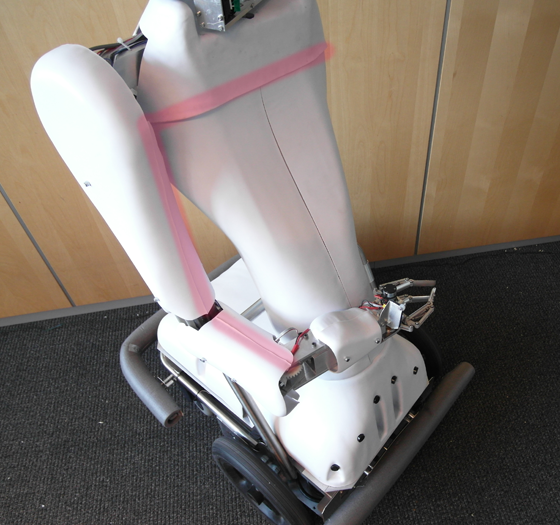
\includegraphics[width=0.5\textwidth]{Images/nonconnectingmodelsurfaces.png}}
	\caption{The red lines indicate places where the covers do not connect well.}
	\label{fig:connect}
\end{figure}

\subsection{Colour design}

Based on a collage of the environment of the intended users a colour study was made. A soft pastel-like color was chosen because it is a color that matches with the colours of the home and it is not a pushy color that makes Eva too crowded – this would contrast with her desired familial product character. Some of the variants (desirable and undesirable) are shown to illustrate the effect of certain colors on the product character. See figure \ref{fig:character} .

This is the final color chosen for Eva \ref{fig:sw_fullrender} . Due to time constraints we have decided not to colour her yet and due to the contrast with the TU Delft logo it is decided that Eva will not be coloured at all.
 
\begin{figure}[h]
	\centering
	\mbox{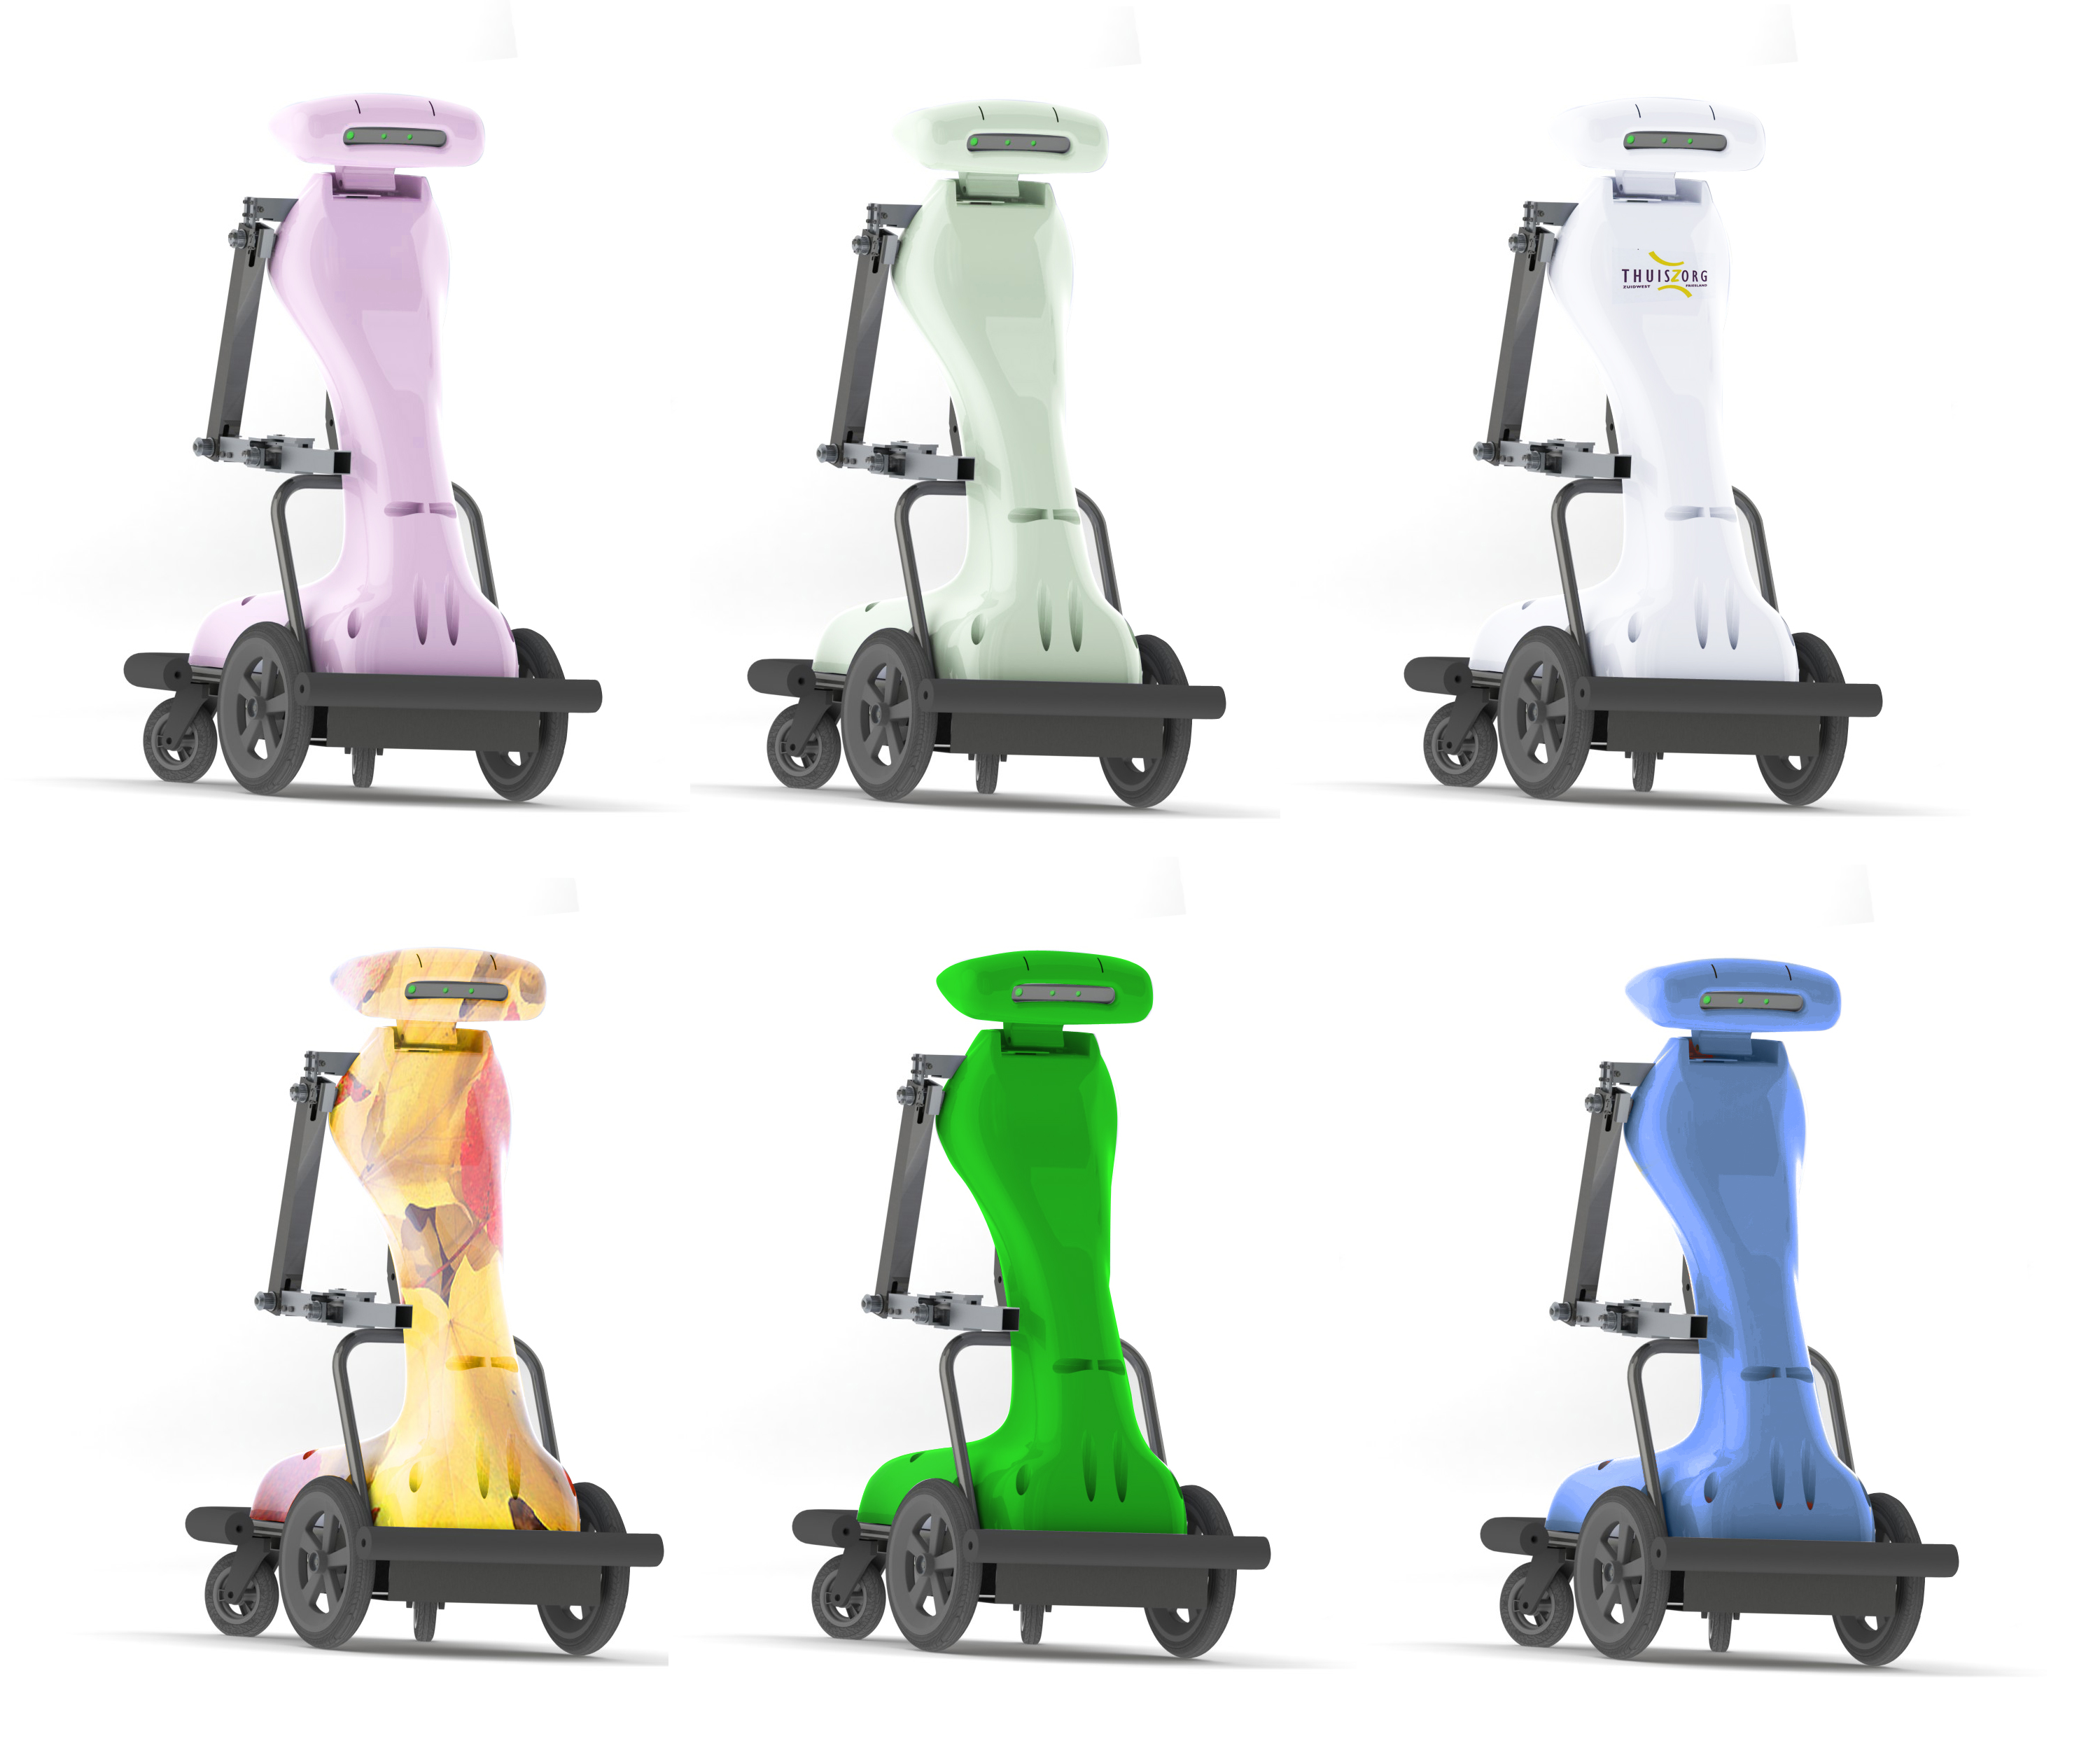
\includegraphics[width=0.5\textwidth]{Images/colorstudy.png}}
	\caption{A study on different colours for Eva.}
	\label{fig:character}
\end{figure}

\begin{figure}[h]
	\centering
	\mbox{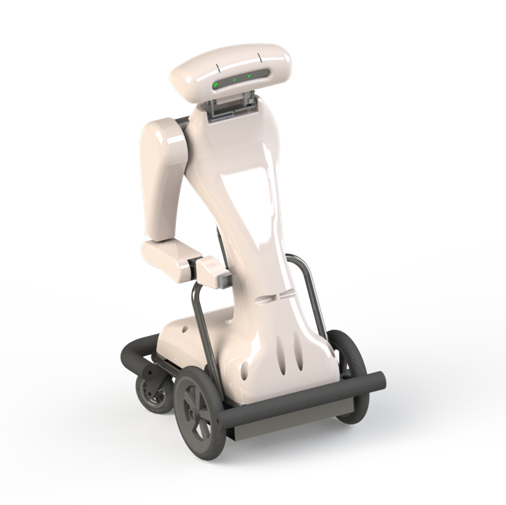
\includegraphics[width=1\textwidth]{Images/SW_fullrender.png}}
	\caption{Full render of Eva in the chosen colour.}
	\label{fig:sw_fullrender}
\end{figure}

\end{document}